\documentclass[main]{subfiles}


\begin{document}
\newpage
\section{Training Methods for Deep ANNs}
\subsection{Recap: Supervised Learning in ANNs}

\begin{figure}[H]
		\centering
		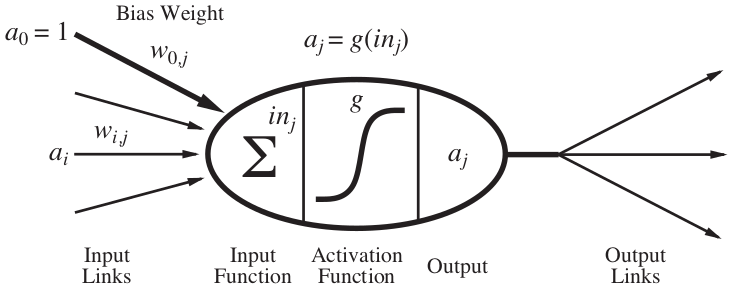
\includegraphics[width=0.8\linewidth]{02_TrainingMethodsForDeepANNs/figures/neuron.png}
		\caption{Simple mathematical model of a hidden neuron: From left to right: Input links constitute of weights coming from previous neurons and from a bias term. The input function, here a sum, bundles the weights. The activation function performs a nonlinear mapping of the input to a output value, which is subsequently passed on to the next neuron.}
		\label{fig:neuron}
	\end{figure}
	
	An artificial neural network (ANN) is a computational model that is vaguely inspired by the biological network of neurons constituting the brain of vertebrates. It can be used as a trainable classifier of data points. Similarly to the biological analogue, it consists of a set of computing units, or \textbf{neurons} and of directed links connecting them. The strength and sign of a link is given through its \textbf{weight}. The neurons take in a set of inputs and produce an output based on a given \textbf{input function} and a given non-linearity, the \textbf{activation function}. A schematic overview of a neuron is given in \cref{fig:neuron}\footnote{Figure and caption adapted from "Russel, AI: A Modern Approach"}. If we bundle many neurons to a layer, and then connect multiple layers by linking the neuronal output of each layer to the neuronal input of the next layer, we get a deep neural network structure, where we differentiate between the input layer, the output layer and the in-between-laying hidden layers. Based on data on the input layer, the network will perform a \textbf{forward-pass} of the information and make a prediction (this can be a classification or regression). During \textbf{training}, the prediction is then compared with the ground-truth, or label, of the data. A \textbf{loss} is calculated based on a difference-norm between the prediction and the true label of the data point. Subsequently, weights of the network are updated. If \textbf{back-propagation} is used, which is the most common algorithm for supervised learning of ANNs, the derivative of the loss with respect to each weight is obtained, the information passed backwards and the weights adjusted accordingly. 
	
	\paragraph{}
	\noindent
	The above described concept can be formulated mathematically. A network with $L$ layers can be defined as 
	
	\begin{equation}
	\bm{h}^j = \sigma^j(W^j\bm{h}^{j-1}) = \sigma^j(\bm{z}^j),\ j=1, ..., L ,
	\end{equation}
	where $\bm{h}^{j}$ is the state of the j-th hidden layer and $\bm{z_i}^j = \sum_{k=0}^{N^j} w_{ik}^j h_i^{j-1}$ the input for the $i$-th neuron in the j-th hidden layer.  $\bm{h}^L$ is the output layer and $\bm{h}^0=\bm{x}$ the input layer. The forward-mapping is defined by the non-linear activation function $\sigma^j$, from which a set of commonly used examples are illustrated in \cref{fig:activation}, and the weight vector $W^j$. Most often, the bias term of the j-th layer $w_{0}^{j}$ is included in the weight vector, thus $W^j = (w_{0}^{j}, w_{1}^{j}, ..., w_{N}^{j})$ defines the weight vector of a layer containing $N^j$ neurons. 
	\begin{figure}[t]
		\centering
		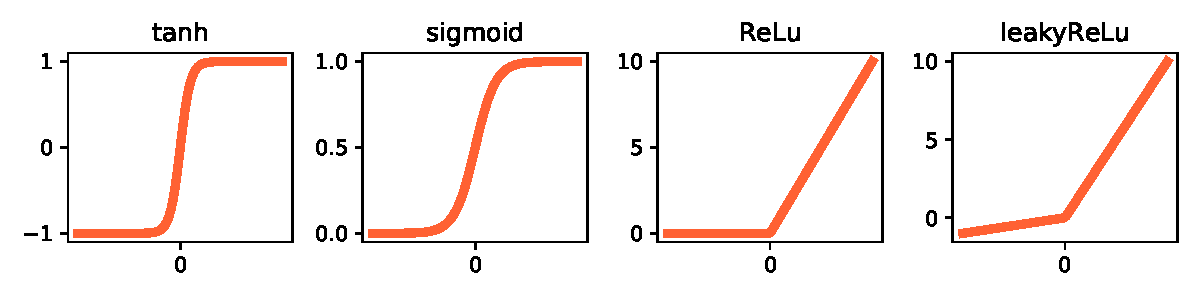
\includegraphics[width=0.99\linewidth]{02_TrainingMethodsForDeepANNs/figures/activations.pdf}
		\caption{Common activation functions: a) $\tanh(x)$ b) $sigmoid(x)$ c) $ReLu(x)$ d) $leakyReLu(x)$}
		\label{fig:activation}
	\end{figure}
	
	
	\noindent
	Now, let's fix the network architecture, meaning the number of neurons, the wiring scheme and the activation $\sigma^j$, and define the network parameters as all the weights $w_{i}^{j}$. If we define all parameters between layer $j$ and $l$ ($0 \leq j < l \leq L$) as $\theta^{j,l}_W = {W^k, k=j+1,...,l}$, we can write the l-th layer $\bm{h^l}$ as a function of the j-th layer $\bm{h^j}$, given the parameters $\theta^{j,l}_W$:
	\begin{equation}
	\bm{h^l} = \bm{h^l}(\bm{h^j}; \theta^{j,l}_W)
	\end{equation}
	%
	For a given data set $(\bm{x}, \bm{y})=((\bm{x_1}, \bm{y_1}), ..., (\bm{x_D}, \bm{y_D}))$, a global loss function $\mathcal{L}(\bm{h}^L(\bm{x}; \theta^{0,L}_W), \bm{y})$ gives a measure of the difference between the network output $\bm{h^L}(\bm{x}; \theta^{0,L}_W)$ and the label $y$. During training, the goal is to minimize the expectation value of the global loss $\mathbb{E}_p\{\mathcal{L}(\bm{h}^L(\bm{x}; \theta^{0,L}_W), \bm{y}) \}$ based on a data distribution $p(\bm{x}, \bm{y})$. Common loss functions are the \textbf{mean-squared-error} (MSE) for regression:
	%
	\begin{equation}
	\mathcal{L}_{MSE}(\bm{h}^L(\bm{x}; \theta^{0,L}_W), \bm{y}) = \frac{1}{2D} \sum_{i=1}^D(\bm{h}^L(\bm{x_i}; \theta^{0,L}_W) - \bm{y_i})^2,
	\end{equation}
	%		
	and the \textbf{cross-entropy loss} (CE) for classification with $C$ classes:
	%
	\begin{equation}
	\mathcal{L}_{CE}(\bm{h}^L(\bm{x}; \theta^{0,L}_W), \bm{y}) = - \sum_{c=1}^C \bm{y_c} \log{\bm{h}_c^{L}(\bm{x_c}; \theta^{0,L}_W)} 
	\end{equation}
	%
	%
	\noindent
	If the back-propagation algorithm is used, updating the weights is done by taking the derivatives of the loss $\mathcal{L}(\bm{h}^L(\bm{x}; \theta^{0,L}_W), \bm{y})$ with respect to all weights $\theta^{0,L}_W$: 
	\begin{equation}
	w^{j,l}[t+1] = w^{j,l}[\ t\ ] - \eta \frac{\partial \mathcal{L}(\bm{h}^L(\bm{x}; \theta^{0,L}_W), \bm{y}) }{\partial w^{j,l}}
	\end{equation}
	%
	%
	The introduced \textbf{learning-rate} factor $\eta$ does in general not need to be constant, thus it can be adaptive over time. 
	
\subsection{Backpropagation}
\subsubsection{Introduction}
Backpropagation (BP) is a widely used algorithm in training feedforward neural networks for supervised learning\footnote{Rumelhart\&Hinton, "Learning representations by back-propagating errors", 1986}. It computes the gradient of the loss function with respect to the weights of the network for a single input/output example, and does so efficiently, unlike a naive direct computation of the gradient with respect to each weight individually. This efficiency makes it feasible to use gradient methods for training multilayer networks, updating weights to minimize loss; gradient descent, or variants such as stochastic gradient descent, are commonly used. The backpropagation algorithm works by computing the gradient of the loss function with respect to each weight by the chain rule, computing the gradient one layer at a time, iterating backwards from the last layer to avoid redundant calculations of intermediate terms in the chain rule; this is an example of dynamic programming\footnote{\url{https://en.wikipedia.org/wiki/Backpropagation}}.

\subsubsection{Method}
We want to calculate the weight error, which is the gradient of the loss with respect to the input of the neuron $j$ of the $l$-th layer $z_j^l$:

\begin{equation}
    \delta_j^l = \frac{\partial \mathcal{L}}{\partial z_j^l}
\end{equation}

First we calculate the gradient with respect to the ultimate layer $L$:

\begin{equation}
    \delta_j^L = \frac{\partial \mathcal{L}}{\partial z_j^L} =  \frac{\partial \mathcal{L}}{\partial h_j^L}\frac{\partial h_j^L}{\partial z_j^L} = \frac{\partial \mathcal{L}}{\partial h_j^L} \sigma'(z_j^L)
\end{equation}

Then, we calculate the gradient with respect to an intermediate layer $l$:

\begin{equation}
    \delta_j^l = \frac{\partial \mathcal{L}}{\partial z_j^l} =  \frac{\partial \mathcal{L}}{\partial z_j^{l+1}}\frac{\partial z_j^{l+1}}{\partial z_j^l} = \delta_j^{l+1} \frac{\partial z_j^{l+1}}{\partial z_j^l} = \sum_k \delta_j^{l+1} w_k^{l+1} \sigma'(z_j^l)
\end{equation}

We note, that the gradient can also be written with a dependency to the weight (??! WHY is that? The first step does not make sense to me, the second one is mathematically not sound (flipping the derivation)):

\begin{equation}
    \delta_j^l = \frac{\partial \mathcal{L}}{\partial z_j^l} = \frac{\partial \mathcal{L}}{\partial w_k^l} \frac{\partial w_k^l}{\partial z_j^l} = \frac{\partial \mathcal{L}}{\partial w_k^l} \frac{1}{h_k^{l-1}}
\end{equation}

Thus, we arrive at the recursive form

\begin{equation}
    \frac{\partial \mathcal{L}}{\partial w_k^l} = h_k^{l-1} \delta_j^l, 
\end{equation}

which gives us the weight update equation as follows:

\begin{equation}
    {w'}_k^l = w_k^l - \eta \Delta w_k^l= w_k^l - \eta \frac{\partial \mathcal{L}}{\partial w_k^l} = w_k^l - \eta h_k^{l-1} \delta_j^l,
\end{equation}

where $\eta$ is the learning rate. 

\subsubsection{Drawbacks}

\begin{itemize}
    \item BP might not be optimal, in particular to train generative models.
    \item BP is not fully local and computation is not easy to parallelize.
    \item BP needs to store all network activations for the BP steps.
    \item Understanding DNN training and optimization methods might provide a different angle to understand learning in biological networks in the Brain. 
    \item Given that the functionality of DNNs is reflected by biological networks the different variants of DNN training even provide testable hypothesis that neuroscience research can test.
    \item Biological plausibility issues, by Bengio\footnote{Lee\&Bengio et al, "Difference Target Propagation", 2015}:
    \begin{enumerate}
        \item The back-propagation computation is purely linear, whereas biological neurons interleave linear and non-linear operations.
        \item If the feedback paths were used to propagate credit assignment by back-propagation, they would need precise knowledge of the derivatives of the non-linearities at the operating point used in the corresponding feedforward computation.
        \item Similarly, these feedback paths would have to use exact symmetric weights (with the same connectivity, transposed) of the feedforward connections.
        \item Real neurons communicate by (possibly stochastic) binary values (spikes)
        \item The computation would have to be precisely clocked to alternate between feedforward and back-propagation phases.
        \item It is not clear where the output targets would come from.
    \end{enumerate}

\end{itemize}




\subsection{Feedback Alignment}
\subsubsection{The Method}
From a biological perspective, one of the biggest issues with backpropagation is that it uses the same weights for the forward and the backward pass. This is tackled with a learning method called feedback alignment\footnote{Lillicrap, "Random synamptic feedback weights support error backpropagation for deep learning", 2016}. Instead of using the transposed weight matrix $W^T$for the backward pass, it uses a matrix of randomly initialized and fixed weights $B$. On simple examples (such as MNIST), the method has been shown to work almost as well as regular back-propagation. The original illustrations and caption can be seen in \cref{fig:feedbackalignment}. We note the change in weight update:
\paragraph{Backpropagation}
\begin{equation}
    \Delta w_k^l = h_k^{l-1} {\delta_{BP}}_j^l = h_k^{l-1} \sum {\delta_{BP}}_j^{l+1} w_{j k}^{l+1} \sigma'(z_j^l)
\end{equation}
\paragraph{Feedback Alignment}
\begin{equation}
    \Delta w_k^l = h_k^{l-1} {\delta_{FA}}_j^l = h_k^{l-1} \sum {\delta_{FA}}_j^{l+1} \beta_{j k}^{l+1} \sigma'(z_j^l)
\end{equation}
where $\bm{\beta}^l$ is a random matrix with fixed weights (does not get updated) belonging to the $l$-th layer.
\begin{figure}[H]
	\centering
	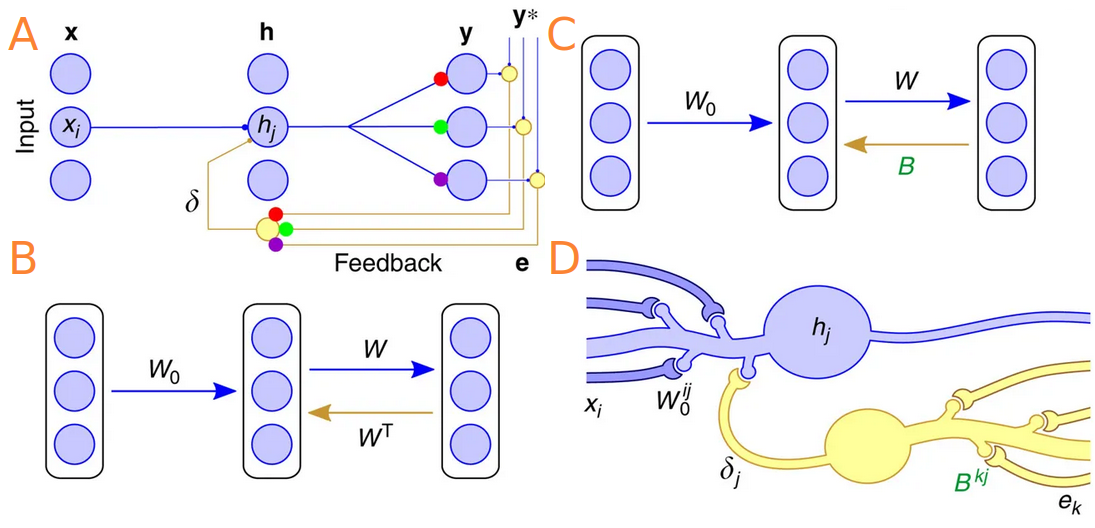
\includegraphics[width=0.99\linewidth]{02_TrainingMethodsForDeepANNs/figures/feedback_alignment.png}
	\caption{\textbf{(A)} The backprop learning algorithm requires that neurons know each others’ synaptic weights, for example, the three coloured synapses on the feedback cell at the bottom must have weights equal to those of the corresponding coloured synapses in the forward path. \textbf{(B)} Backprop computes teaching, or modulator, vectors by multiplying the error vector $\bm{e}$ by the transpose of the forward weight matrix W, that is, $\delta_{BP}=W^T\bm{e}$. \textbf{(C)} Our feedback alignment method replaces $W^T$ with a matrix of fixed random weights, $B$, so that $\delta_{FA}=B\bm{e}$. Thus, each neuron in the hidden layer receives a random projection of the error vector. \textbf{(D)} Potential synaptic circuitry underlying feedback alignment, shown for a single hidden unit (matrix superscripts denote single synapses, see main text for further explanation). This diagram is provide for illustrative purposes. There are many possible configurations that could support learning with feedback alignment, or algorithms like it, and it is this structural flexibility that we believe is important.}
	\label{fig:feedbackalignment}
\end{figure}

\subsubsection{Why does it work?}
Some mathematical reasoning and the convergence proof is shown in the original paper and stated again in a follow-up paper. Intuitively; for FA the feedback weights are fixed, but if the forward weights are adapted, they will approximately align with the pseudo-inverse of the feedback weights in order to make the feedback useful. In some sense, the network learns how to learn, which is pretty dope. 

\subsubsection{Variations of Feedback Alignment}
There are variations of feedback alignment, which show to be useful especially for deeper network architectures. The figure below shows Feedback Alignment (FA), Direct Feedback Alignment (DFA) and Indirect Feedback alignment\footnote{Nøkland, "Direct Feedback Alignment Provides Learning in Deep Neural Networks", 2016} (IFA).  In \cref{fig:bidirect_feedbackalignment} we see the Bi-directional Feedback Alignment\footnote{Luo, "Adaptive Bidirectional Backpropagation: Towards Biologically Plausible Error Signal Transmission in Neural Networks", 2017} (BFA).

\begin{figure}[H]
	\centering
	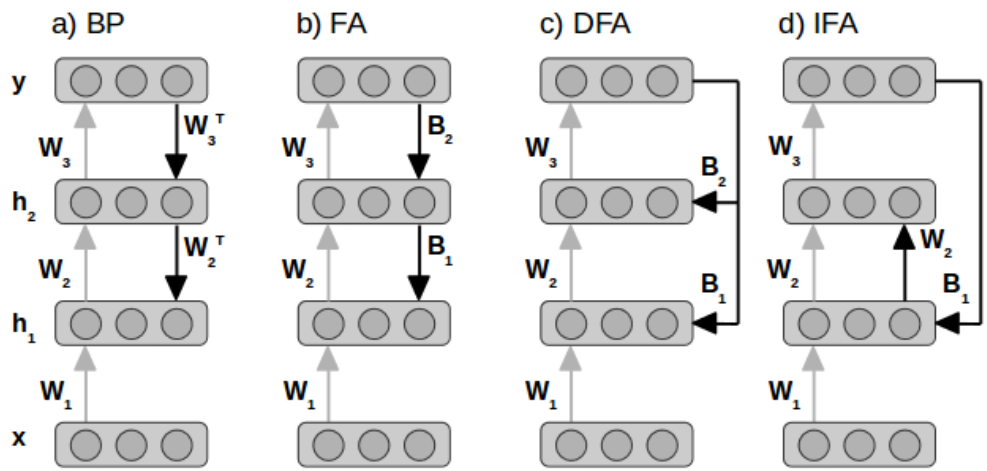
\includegraphics[width=0.99\linewidth]{02_TrainingMethodsForDeepANNs/figures/direct_feedbackalignment.png}
	\caption{Overview of different error transportation configurations. Grey arrows indicate activation paths and black arrows indicate error paths. Weights that are adapted during learning are denoted as $W_i$ , and weights that are fixed and random are denoted as $B_i$. \textbf{(a)} Back-propagation. \textbf{(b)} Feedback-alignment. \textbf{(c)} Direct feedback-alignment. \textbf{(d)} Indirect feedback-alignment.}
	\label{fig:direct_feedbackalignment}
\end{figure}

\begin{figure}[H]
	\centering
	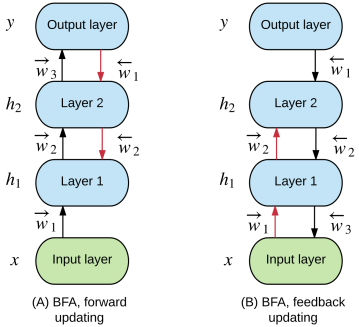
\includegraphics[width=0.6\linewidth]{02_TrainingMethodsForDeepANNs/figures/bidirect_feedbackalignment.png}
	\caption{Bidirectional feedback alignment (BFA). Black arrows represent forward activation paths. Red arrows indicate error (gradient) propagation paths.}
	\label{fig:bidirect_feedbackalignment}
\end{figure}



\subsection{Target Propagation}

\subsubsection{The Method}
The main idea is to compute targets rather than gradients, at each layer\footnote{LeCun, "Learning processes in an asymmetric threshold network", 1986},\footnote{Lee\&Bengio et al, "Difference Target Propagation", 2015}. Like gradients, they are propagated backwards. In a way that is related but different from previously proposed proxies for back-propagation which rely on a backwards network with symmetric weights, target propagation relies on auto-encoders at each layer. Unlike back-propagation, it can be applied even when units exchange stochastic bits rather than real numbers. By its nature, target propagation can in principle handle stronger (and even discrete) non-linearities, and it deals with biological plausibility issues (1), (2), (3) and (4) described above. A sketch of the working principle is shown below. 

\begin{figure}[H]
	\centering
	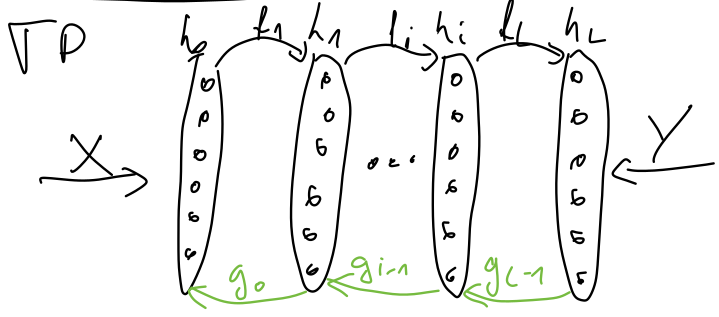
\includegraphics[width=0.7\linewidth]{02_TrainingMethodsForDeepANNs/figures/target_propagation.png}
	\caption{}
	\label{fig:targetprop}
\end{figure}

\paragraph{Forward pass}
\begin{equation}
	\bm{h}^j = f^j(\bm{h}^{j-1}) = \sigma^j(W^j\bm{h}^{j-1}) = \sigma^j(\bm{z}^j),\ j=1, ..., L ,
\end{equation}

\paragraph{Backward pass}
\begin{equation}
	\bm{\hat{h}}^j = g^j(\bm{\hat{h}}^{j+1}),\ j=L-1, ..., 0 ,
\end{equation}
where $\bm{\hat{h}}^j$ is the target of the $j$-th layer and $g^j$ is a function that must approximate the inverse of $f^{j+1}$. The output target is defined as the activation of the output layer tweaked in a direction of lower loss:
\begin{align}
	\bm{\hat{h}}^L &= \bm{h}^L - \hat{\eta}\bm{e}^L\\
	\bm{e}^L &= \frac{\partial \mathcal{L}}{\partial \bm{h}^L}
\end{align}

\paragraph{Learning the forward weights}
Based on the hidden layer targets $\bm{\hat{h}}^j$, local layer losses $\mathcal{L}^j(\bm{h}_{true}^j, \bm{\hat{h}}^j)$ are defined (for example the L2 loss). The forward weights $W^j$ are then updated as follows:

\begin{equation}
    \Delta W^j = -\eta_{f^j} \frac{\partial \mathcal{L}^j(\bm{h}_{true}^j, \bm{\hat{h}}^j)}{\partial W^j}
\end{equation}

\paragraph{Learning the backward mapping}
The backward mapping $g^j$ should approximate the inverse of the forward mapping $f^{j+1}$. Target propagation achieves this by "learning $g^j$" through an autoencoder setting of $f^{j+1}$ (encoder) and $g^j$ (decoder). $g^j$ is parametrized with a non-linear activation function $t^j$ and a backwards weight matrix $\bm{Q}^j$: 
%
\begin{equation}
    g^j(\bm{\hat{h}}^{j+1}) = t^j(\bm{Q}^j\bm{\hat{h}}^{j+1})
\end{equation}
%
The decoder $g^j$ can then be trained via a reconstruction loss:
%
\begin{align}
    \mathcal{L}_{rec}^j(g^j(f^{j+1}(\bm{h}^j)), \bm{h}^j) &= \| g^j(f^{j+1}(\bm{h}^j)) - \bm{h}^j\|^2\\
    \Delta \bm{Q}^j &= -\eta_{g^j} \frac{\partial \mathcal{L}_{rec}^j}{\partial \bm{Q}^i}
\end{align}

The total loss is then composed by the local layer loss and the reconstruction loss of $g^j$ and $(f^{j+1})^{-1}$:

\begin{equation}
    \mathcal{L}^j = \mathcal{L}_{local}^j(\bm{h}_{true}^j, \bm{\hat{h}}^j) + \mathcal{L}_{rec}^j(g^j(f^{j+1}(\bm{h}^j)), \bm{h}^j)
\end{equation}

\subsubsection{Difference Target Propagation}
So far, a vanilla Target Propagation did not seem to be successful at all. The biggest reason is, that the learned function $g^j$ will never be a perfect inverse of $f^{j+1}$ and thus the reconstruction loss always large. Difference Target Propagation\footnote{Lee\&Bengio et al, "Difference Target Propagation", 2015} approached this problem by proposing a correction term in the propagated target $\bm{\hat{h}}^{j}$ that should help in getting rid of the reconstruction error:
%
\begin{equation}
    \bm{\hat{h}}^{j} = g^j(\bm{\hat{h}}^{j+1}) + (\bm{h}^{j} - g^i(\bm{h}^{j+1}))
\end{equation}
%
Note that if $g^j$ is exactly the inverse, then it is the same as vanilla target propagation. An illustration to direct target propagation is shown below.

\begin{figure}[H]
	\centering
	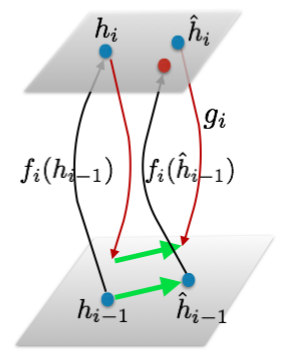
\includegraphics[width=0.45\linewidth]{02_TrainingMethodsForDeepANNs/figures/dtp.png}
	\caption{How to compute a target in the lower layer via difference target propagation. $f^i( \hat{h}^{i-1})$ should be closer to $\hat{h}^i$ than $f^i(h^{i-1})$}
	\label{fig:targetprop}
\end{figure}



\subsection{Local Learning}
There are approaches that train neuronal networks using Local Layer error signals\footnote{Nokland, Training Neural Networks with Local Error Signals, 2019} \footnote{Mostafa, "Deep Supervised Learning Using Local Errors", 2018}. This has the advantages, that activations don't occupy space in memory, and that parallelization becomes easy (each layer in own GPU, train all simultaneously). One can use a combination of Similarity Matching Loss (sim) and Cross Entropy Loss (pred).

\subsection{Questions}
\begin{enumerate}
    \item How could biological neurons differ between FF and BP error signals?
    \item How do biological neurons change their incoming weights (synaptic connections)?
    \item Do biological neurons follow a purely local update rule?
    \item What is the depth (hierarchical layers) of biological neuronal networks of the human/primate visual system?
\end{enumerate}


\end{document}